\documentclass[aspectratio=169]{beamer}
\usepackage[utf8]{inputenc}
\usepackage{amsmath}
%\usepackage[ngerman]{babel}
\usepackage{xcolor}
\usepackage{listings}
%\usepackage[automark]{scrpage2}
\usepackage[]{graphicx, import} 
\usepackage{subfigure}
\usepackage{wrapfig}
\usepackage[scaled]{helvet}
\renewcommand*\familydefault{\sfdefault}
%\usepackage{enumitem}
\usepackage{harvard}
\usepackage{url}
\citationstyle{dcu}
%\setbeamertemplate{footline}[page number]
\usetheme{FHNW}
\usecolortheme{seagull}
\usepackage{multimedia}

\usepackage{hyperref}



\begin{document}
% infos for pdf document settings
\pdfinfo{
/Author (Stefan Blaser, FHNW - IVGI)
/Title (Development of an Acquisition Software 
	for our Image-Based Indoor Mobile Mapping System 
	based on the Robot Operating System (ROS))
/Subject (GeoPython 2017)
/Keywords (ROS, Mobile Mapping, Indoor, Python)}

% infos for title page
\title{\textbf{Development of an Acquisition Software
	for our Image-Based Indoor Mobile Mapping System 
	based on the Robot Operating System (ROS)}}
\subtitle{GeoPython 2017}
\author{Stefan Blaser}
\institute{Institute of Geomatics Engineering}
\date{\today}

% title page
\begin{frame}
 \titlepage
\end{frame}

\section{Introduction}

% Frame 1: Trends in geodata acquisition
  \begin{frame}
   \frametitle{Introduction}
   \begin{columns}[onlytextwidth]
    \begin{column}{0.5\textwidth}
    
    % TODO insert Image (IOT)
    
    \end{column}
    \begin{column}{0.5\textwidth}
    Trends in geodata acquisition:
      \begin{itemize}
       \item outsourcing / crowd-sourcing
       \item IoT
       \item using sophisticated multi-sensor systems
      \end{itemize}
    \end{column}
   \end{columns}
  \end{frame}

% Frame 2: Mobile Mapping
  \begin{frame}
   \frametitle{Introduction}
   \begin{columns}[onlytextwidth]

    \begin{column}{0.5\textwidth}
    Mobile Mapping
      \begin{itemize}
       \item Image-based Mobile Mapping \newline(since 2011 @ FHNW)
       % TODO cite Burkhard et. al (2011)
       \item Spin-off company iNovitas
       \item ``Google Street View''-like service
       \item Measurement functionality
       \item Measurement accuracy:
       \begin{itemize}
        \item relative: ca. $1\, cm$
        \item absolute: ca. $3-5\, cm$ \newline(GNSS accuracy)
       \end{itemize}
      \end{itemize}
    \end{column}
    \begin{column}{0.5\textwidth}
    
     \begin{figure}[h]
       \centering
       \includegraphics[width=5.5cm]{./Abbildungen/mms.png}
       \caption{Mobile Mapping vehicle of FHNW}
       \label{abb:mms}
     \end{figure}
     
    \end{column}
    
   \end{columns}
  \end{frame}

% Frame 3: CTI-Project BIMAGE
  \begin{frame}
   \frametitle{Introduction}
   \begin{columns}[onlytextwidth]

    \begin{column}{0.5\textwidth}
    CTI project ``BIMAGE''
      \begin{itemize}
       \item Main Goal: 
       \begin{itemize}\item Transfer outdoor technology into interior spaces\end{itemize}
       \pause
       \item Deliverables:
       \begin{itemize}
        \item \textbf{Indoor Mobile Mapping System} (IMMS) (absence of GNSS) \pause
        \item Software to follow changes using mobile devices \pause
        \item New navigation concepts for cloud application \pause
        \item Sophisticated photogrammetric image post-processing approaches 
       \end{itemize}
      \end{itemize}
    \end{column}
    \begin{column}{0.5\textwidth}
    \begin{center}
    
\includegraphics[width=0.9\textwidth]{./Abbildungen/FHNW_HABG_10mm.jpg} \\
    % FHNW_HABG_10mm.jpg: 0x0 pixel, 300dpi, 0.00x0.00 cm, bb=
    
\includegraphics[width=0.2\textwidth]{./Abbildungen/iNovitas_Logo.png} \\
    % iNovitas_Logo.png: 0x0 pixel, 300dpi, 0.00x0.00 cm, bb=
    
\includegraphics[width=0.7\textwidth]{./Abbildungen/F&E_Absender_Dritte_Un_D_1200.png}
% F&E_Absender_Dritte_Un_D_1200.png: 0x0 pixel, 300dpi, 0.00x0.00 cm, bb=
    \end{center}
    
    \end{column}
    
   \end{columns}
  \end{frame}


\section{Software Requirements}

  \begin{frame}
   \frametitle{Requirements for the acquisition software}
   \begin{columns}[onlytextwidth]
    \begin{column}{0.5\textwidth}
    
    \begin{figure}[h]
      \centering
      \includegraphics[height=6.05cm]{./Abbildungen/imms.png}
      %\caption{IMMS prototype}
      \label{abb:imms}
    \end{figure}

    \end{column}
    \begin{column}{0.5\textwidth}
      \begin{itemize}
       \item IMMS prototype (see figure)  
       \begin{itemize}
        \item panorama camera
        \item laser scanner
        \item IMU (tactical grade)
        \item GNSS
	\item weight: $30\,kg$ ($66.1\, lbs$)
	\item hardware changes necessary
       \end{itemize}
       \pause
       \item Modular software architecture
       \item Free open source software (FOSS)
       \item Existing modules for hardware support
      \end{itemize}
    \end{column}

   \end{columns}
  \end{frame}

\section{Robot Operating System (ROS)}

  \begin{frame}
   \frametitle{Robot Operating System (ROS)}
   \begin{columns}[onlytextwidth]
    \begin{column}{0.5\textwidth}
    
      \begin{itemize}
       \item Software framework for robots 
       \item Free and Open-Source 
       \item Graph-based communication layer 
       \item Collection of tools and libraries 
       \item Multi-lingual 
       \begin{itemize}
	\item C++
	\item \textbf{Python} 
       \end{itemize}
       \item \url{www.ros.org}
      \end{itemize}
    
    \end{column}
    \begin{column}{0.5\textwidth}

    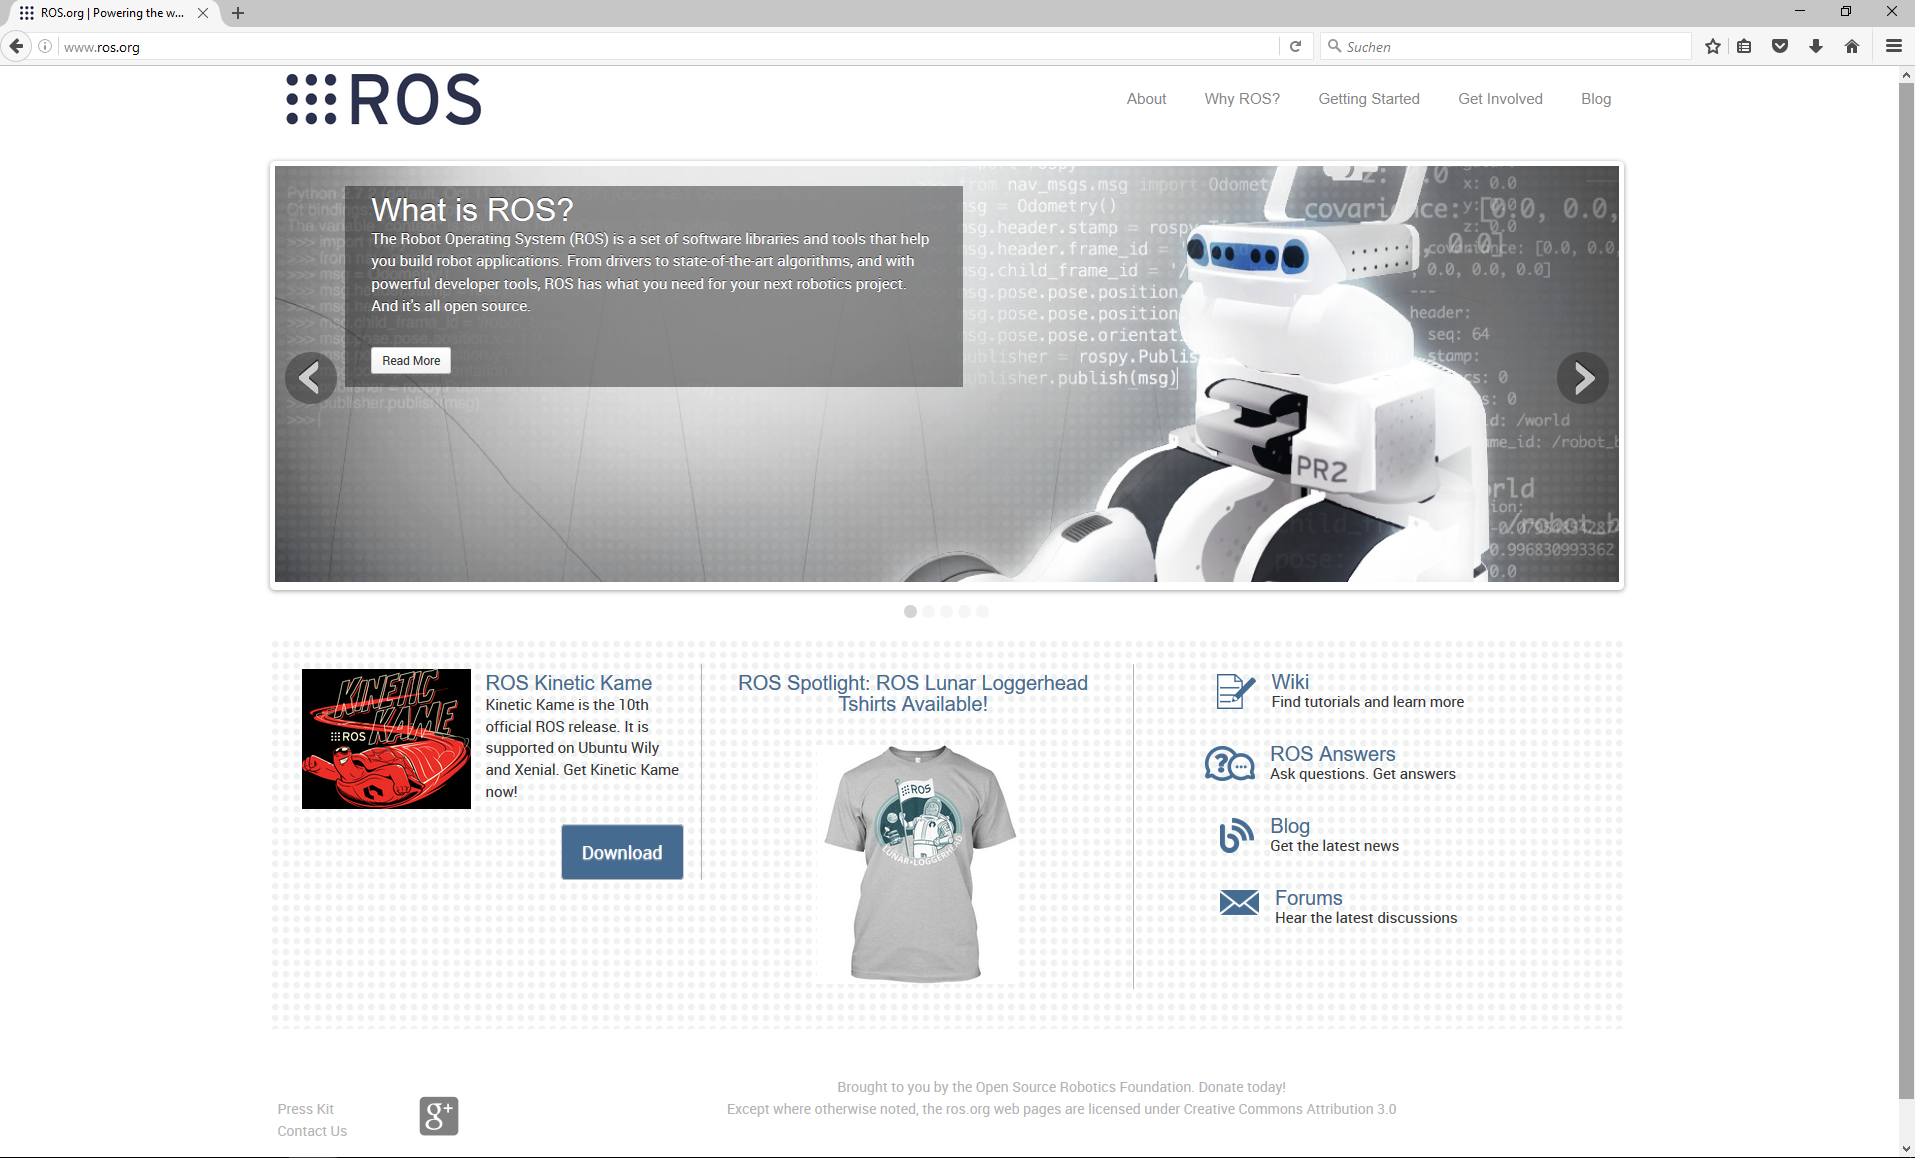
\includegraphics[width=1.5\textwidth]{./Abbildungen/ros_screenshot.png}
    % ros_screenshot.png: 0x0 pixel, 300dpi, 0.00x0.00 cm, bb=
    
    \end{column}
   \end{columns}
  \end{frame}

  \begin{frame}
   \frametitle{Graph-based communication layer}
   \begin{columns}[onlytextwidth]
    \begin{column}{0.5\textwidth}
    
      \begin{description}
       \item [\textbf{Node}] software module, process
       \item [\textbf{Messages}] data in a predefined structure
       \item [\textbf{Topic}] where messages go through
       \item [\textbf{Service}] allows synchronous communication (request / response)
      \end{description}
       
    \end{column}
    \begin{column}{0.5\textwidth}

      \begin{figure}[h]
	\centering
	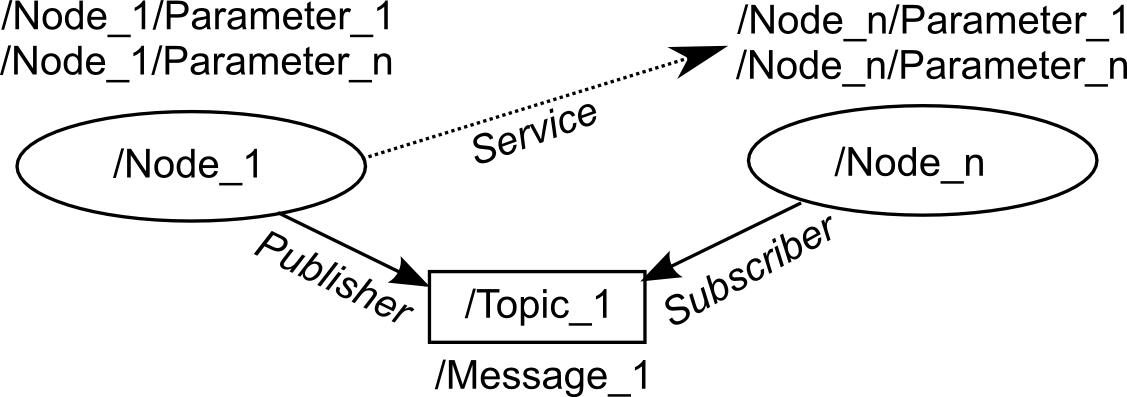
\includegraphics[width=\textwidth]{./Abbildungen/ROS-Graph-basic.png}
	% ROS-Graph-basic.png: 0x0 pixel, 300dpi, 0.00x0.00 cm, bb=
	\caption{ROS communication principle}
	\label{abb:graph}
      \end{figure}
    \end{column}
   \end{columns}
  \end{frame}

\section{Implemented Acquistion Software}

  \begin{frame}
   \frametitle{Acquisition software design}
    
    \begin{figure}[h]
      \centering
      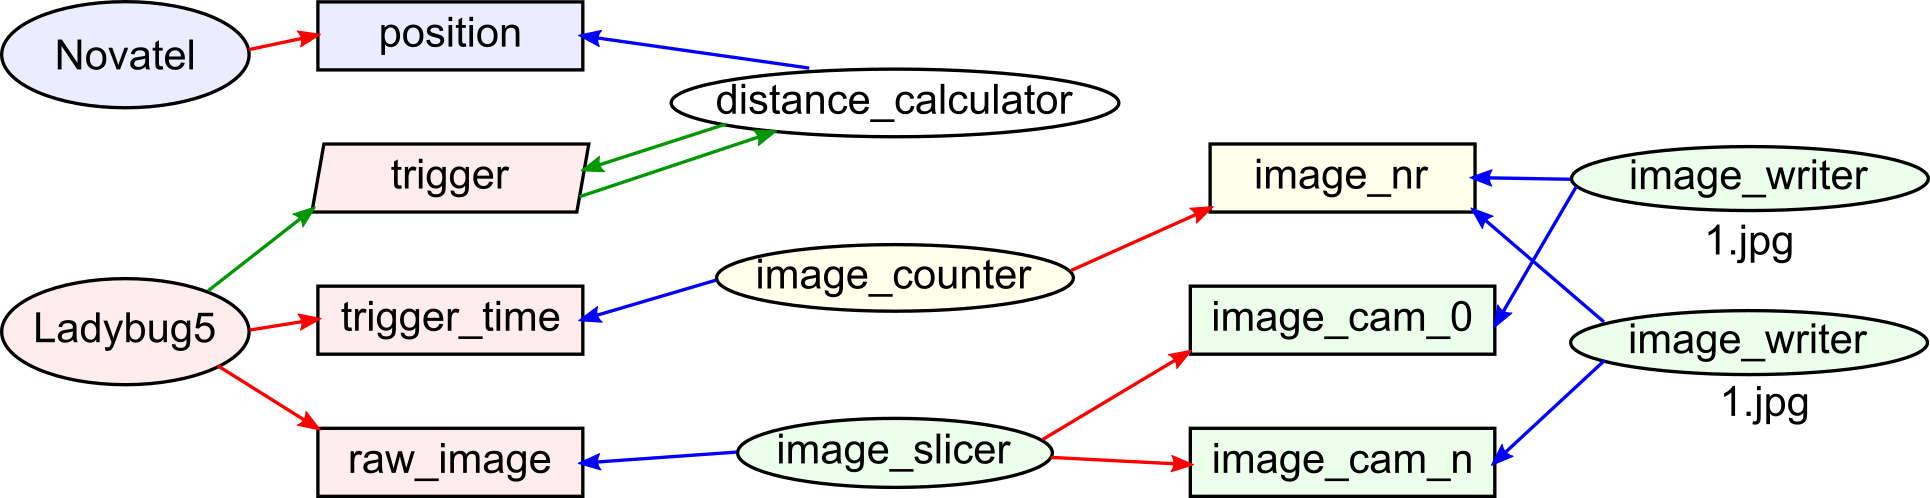
\includegraphics[width=13.5cm]{./Abbildungen/ROSImageCapturing.png}
      % ROSImageCapturing.png: 0x0 pixel, 300dpi, 0.00x0.00 cm, bb=
      \caption{Graph-based software design of the image acquisition part}
      \label{abb:ROSImageCapturing}
    \end{figure}

  \end{frame}

% Python listings image event counter
\defverbatim[colored]\lstOne{
  \begin{lstlisting}[language=python, basicstyle=\ttfamily, keywordstyle=\color{blue}]
#!/usr/bin/env python
import rospy
from std_msgs.msg import *

class ImageEventCounter():
    [...]

def main():
    [...]

if __name__ == '__main__':
    main()
  \end{lstlisting}
}
\defverbatim[colored]\lstTwo{
  \begin{lstlisting}[language=python, basicstyle=\ttfamily, keywordstyle=\color{blue}]
def main():
    rospy.init_node("ImageEventCounter", 
                    anonymous=True)
    image_event_counter_node = ImageEventCounter()
    try:
        rospy.spin()
    except KeyboardInterrupt:
        pass
  \end{lstlisting}
}
\defverbatim[colored]\lstThree{
  \begin{lstlisting}[language=python, basicstyle=\ttfamily, keywordstyle=\color{blue}]
class ImageEventCounter():
    def __init__(self):
        # read out parameter
        self.counter = \
            rospy.get_param('counter_start', 0)
        mark_1_time_topic_name = \
            rospy.get_param('subscriber_name', 
                            '/mark_1_time')
        n_mark_1_time_topic_name = \
            rospy.get_param('publisher_name', 
                            '/n_mark_1_time')
	[...]
  \end{lstlisting}
}
\defverbatim[colored]\lstFour{
  \begin{lstlisting}[language=python, basicstyle=\ttfamily, keywordstyle=\color{blue}]
class ImageEventCounter():
    def __init__(self):
	[...]
	self.mark_1_time_sub = \
	    rospy.Subscriber(mark_1_time_topic_name,
                             Time,
                             self.mark_1_time_callback)
        self.mark_1_time_pub = \
	    rospy.Publisher(n_mark_1_time_topic_name,
                            UInt32,
                            queue_size=1)
    def mark_1_time_callback(self, time):
        [...]
  \end{lstlisting}
}
\defverbatim[colored]\lstFive{
  \begin{lstlisting}[language=python, basicstyle=\ttfamily, keywordstyle=\color{blue}]
class ImageEventCounter():
    def __init__(self):
	[...]
    def mark_1_time_callback(self, time):
        self.counter += 1
        self.mark_1_time_pub.publish(UInt32(\
                                     self.counter))
  \end{lstlisting}
}

\begin{frame}
 \frametitle{Node ImageEventCounter}
 \lstOne
\end{frame}

\begin{frame}
 \frametitle{Node ImageEventCounter}
 \lstTwo
\end{frame}

\begin{frame}
 \frametitle{Node ImageEventCounter}
 \lstThree
\end{frame}

\begin{frame}
 \frametitle{Node ImageEventCounter}
 \lstFour
\end{frame}

\begin{frame}
 \frametitle{Node ImageEventCounter}
 \lstFive
\end{frame}

\section{Conclusion and Outlook}

\end{document}
